\documentclass[11pt]{article}
\usepackage[margin=0.9in]{geometry}
\usepackage{graphicx}
\usepackage{url}
\usepackage{mathtools}
\usepackage{amsmath}
\fboxsep=1mm%padding thickness
\fboxrule=1pt%border thickness
\usepackage{listings}
\usepackage{color}

\definecolor{dkgreen}{rgb}{0,0.6,0}
\definecolor{gray}{rgb}{0.5,0.5,0.5}
\definecolor{mauve}{rgb}{0.58,0,0.82}

\lstset{frame=tb,
  language=Java,
  aboveskip=3mm,
  belowskip=3mm,
  showstringspaces=false,
  columns=flexible,
  basicstyle={\small\ttfamily},
  numbers=none,
  numberstyle=\tiny\color{gray},
  keywordstyle=\color{blue},
  commentstyle=\color{dkgreen},
  stringstyle=\color{mauve},
  breaklines=true,
  breakatwhitespace=true,
  tabsize=3
}

\begin{document}
\begin{titlepage}
	\newcommand{\HRule}{\rule{\linewidth}{0.3mm}}	
	\center
	\vfill\vfill
	
\includegraphics[width=0.6\textwidth]{logoUJM.png}\\[2cm]	
	\textsc{\LARGE Data Mining}\\[1.0cm]
	\textsc{\Large Report}\\[0.5cm]	
	\HRule\\[0.4cm]
	{\LARGE\bfseries Divvy Bike Sharing Data Mining in R}\\[0.4cm]
	\HRule\\[0.8cm]	
	\begin{minipage}{0.4\textwidth}
		\begin{flushleft}
			\large
			\textit{Student}\\
			Maliha \textsc{Ashraf (MLDM)}
		\end{flushleft}
	\end{minipage}
	~
	\begin{minipage}{0.4\textwidth}
		\begin{flushright}
			\large
			\textit{Supervisor}\\
			Fabrice \textsc{Muhlenbach}
		\end{flushright}
	\end{minipage}
	\vfill\vfill\vfill	
	{\large 17 March 2019}	
	\vfill
\end{titlepage}
\pagenumbering{arabic}
\newpage

\section{Problem Understanding}
Bike/Bi-cycle Sharing systems are becoming popular through out the world. These systems allow users to rent a bike for a short period of time(for eg:30mins). Many bike-sharing systems have made the data public. DivvyBikes is also one of them, which is a bike sharing company in Chicago, USA. For a bike-sharing company, it is very important for them to know the usage of bikes at certain stations. In this report I will use this data to analyse what factors affect the number of bikes rented per station and then try to predict the count.
\newline\newline
Also, as this dataset gives the trip details(location,duration,time), it is possible that if there is some incident in the city which affects the traffic, we can observe it in the dataset. So I will try to see if I can detect something for a real incident in Chicago.

\section{Data Understanding}
The data used in this report has been taken from divvybikes.com[1]. They release the data twice a year, breaking it down in 4 quarters; Q1(Jan-Mar), Q2(Apr-Jun), Q3(Jul-Sept) and Q4(Oct-Dec). For this report, the data for the year 2018 has been used.
\newline\newline
No. of records: Q1: 387145, Q2: 1059681, Q3: 1513570, Q4: 642687 \newline
No. of attributes: 12
\newline\newline
The attributes of the dataset are defined below:
\begin{enumerate}
   \item trip\_id: unique ID for every trip | 20983530 |
   \item start\_time: Trip start date and time | 10/1/2018  12:01:17 AM |
   \item end\_time: Trip end date and time | 10/1/2018  12:29:35 AM |
   \item bikeid: unique ID of the bike used during a single trip | 4551 |
   \item tripduration: duration of the trip in seconds | 1,698.00 |
   \item from\_station\_id: Trip start station id | 85 |
   \item from\_station\_name: Trip start station name | Michigan Ave \& Oak St |
   \item to\_station\_id: Trip end station id <166 |
   \item to\_station\_name: Trip end station name | Ashland Ave \& Wrightwood Ave |
   \item usertype: Subscriber(Member, Single Ride, and Explore Pass), Customer
   \item gender: Male, Female for subscribers and empty for customers
   \item birthyear: 4-digit number for subscribers' birth year | 1992 |
\end{enumerate}
User is kept annonymous in this dataset. However, if the trip is made by a subscriber, then User Type, Gender and Birth Year is included.

\section{Data Preparation}
\begin{enumerate}
\item Read the data files of allquarters through the .csv file using read.csv() method
\item Combined the data in one dataframe through rbind() method and saved the dataframe in csv file.
\item The start\_time has both date and time.Separated them by the use of as.POSIXct() method.Resulting new features are: Start\_Date, Start\_Time. Deleted start\_time.
\item Extracted hour from Time and store in separate column, because I need it in analyzing the data by the hour.
\begin{lstlisting}
Trips_2018$start_hour =  as.numeric(substr(Trips_2018$Start_Time, 1, 2))
\end{lstlisting}
\item  Extracted weekday and month from Start\_Date and store in separate column,to be used later, by using weekdays() and months() methods.
\begin{lstlisting}
Trips_2018$day <- weekdays(Trips_2018$Start_Date)
Trips_2018$month <- months(Trips_2018$Start_Date)
\end{lstlisting}
\item Downloaded weather data from the official website of chicago weather updates[2] and load it in a dataframe. Changed the format of the date column to match the Start\_Date column of our trips data.
\begin{lstlisting}
weatherdata = read.csv("weather_Q3_2018.csv")
weatherdata$Start_Date = gsub("-","/",weatherdata$date)
weatherdata$Start_Date = strptime(as.character(weatherdata$Start_Date), "%Y/%m/%d")
weatherdata$Start_Date = format(weatherdata$Start_Date,"%m/%d/%Y")
weatherdata$date <- NULL
\end{lstlisting}
Replaced the missing numeric values of by the mean of the column.
\begin{lstlisting}
for (j in 1:ncol(weatherdata)){ 
  weatherdata[is.na(weatherdata[, j]), j] <- mean(weatherdata[, j], na.rm = TRUE) 
  }
\end{lstlisting}
\item Merged Trips data and weather data on the column Start\_Date. From the weather data we only need the average temparature, precipitation and snow fall information for a day.
\begin{lstlisting}
tripsData = merge(x = Trips_2018, y = weatherdata[ , c("Start_Date","average","percipitation","new_snow","snow_depth")], by.x = "Start_Date", by.y = "Start_Date", all.y=TRUE)
\end{lstlisting}
\item At this point, I am saving the fnal merged data to .csv file and will import it direclty for all my following work.
\begin{lstlisting}
write.csv(tripsData,"tripsData")
\end{lstlisting}
\end{enumerate}
\section{Exploratory Analysis}
Bike-Sharing datasets are very interesting to explore. They tell you a lot about the traffic situations in a city. I tried to check if I can validate the traffic incidents happening in the city through the dataset. I tried different incident news and approaches. Sometimes the hours of the incidents were such that it didn't cause much difference to the stats of the data or the incident was not much impactful to appear on graph. However, after some work I finally detected something. This event happened on Tuesday morning impacting the rush hours of the city resulting in  a sudden and considerable (almost double) drop of number of trips as compared to other tuesday mornings.\newline\newline

\includegraphics[width=1\linewidth]{nbcc.png}\newline
\begin{lstlisting}
hfilter <- c("8") # the impacted hour
dfilter<- c("09/11/2018","09/18/2018","09/25/2018","10/02/2018","10/09/2018","10/16/2018",
					"10/23/2018","10/30/2018")
tuesdayData = tripsData[tripsData$Start_Date %in% dfilter 
									& tripsData$start_hour %in% hfilter , ]
graphdata = sqldf("select Start_Date, COUNT(*) from tuesdayData GROUP BY Start_Date")
ggplot(data=graphdata, aes(x=Start_Date, y=Trips_Count, group=1)) + 
geom_line() + 
geom_point()
\end{lstlisting}
\begin{figure}[h!]
  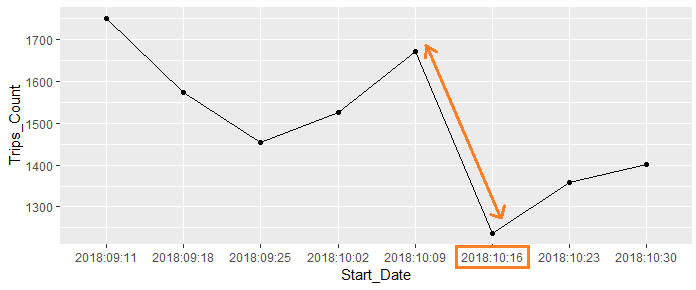
\includegraphics[width=1\linewidth]{plot.png}
  \caption{16th October 2018 Incident}
\end{figure}

Now, I will explore the data for the prediction of number of trips. From the data provided by DivvyBikes, the obvious features could be day and month. So, I will first plot to see how the trip count is affected by these two.

\begin{figure}[h!]
  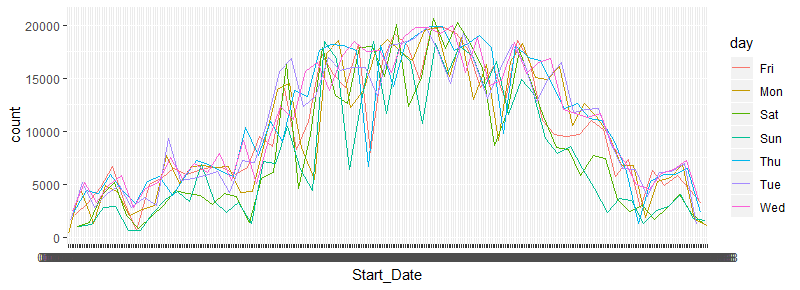
\includegraphics[width=1\linewidth]{Rplot1.png}
  \caption{Factors affecting Trips Count}
\end{figure}

This plot is for whole year 2018, with dates on x-axis and trips count on y-axis and days are indicated by unique colors. We can deduce two things from this plot: 
\begin{enumerate}
\item The trip counts are low at the start of the year, maximum around the middle and again low towards the end of the year. From this, we can deduce that the seasons have an impact on trips count, i.e, around spring and summers the trips are more in quantity and low around the winters. So I will consider the weather data whle modeling.
\item The trip count is affected by what day-of-the-week is it? We can see that there is a considerable drop in counts over the weekends. Below is the graph for only month of December to see clearly.
\begin{figure}[h!]
  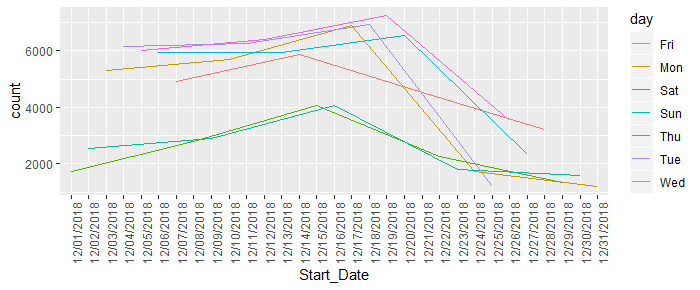
\includegraphics[width=1\linewidth]{Rplot.png}
\end{figure}

If we look at Figure 2 again closely, we can see that this difference between weekdays and weekends is also seasonal. May be people like to stay-in on weekends in winters contrary to summer days.
\end{enumerate}

\section{Modeling}
We need to predict the number of bikes needed at a certain station at certain hour. For this report, I have selected the station with the highest number of trips in 2018.
\begin{lstlisting}
stationsCount = sqldf("Select from_station_id,count(*) from Trips_2018 GROUP BY from_station_id")
stationData = Trips_2018[Trips_2018$from_station_id==35,]
\end{lstlisting}
As we saw in exploratory analysis that month, day and weather are impacting the trips count, so I have selected the relevant features according to them.
\begin{lstlisting}
modeldata = sqldf("Select month,day,start_hour,average,percipitation,new_snow,snow_depth,count(*) from stationData GROUP BY from_station_id, Start_Date,start_hour")
\end{lstlisting}
For month, day and start\_hour I have performed one-hot-encoding as the features are not numeric ranges.
\begin{lstlisting}
modeldata$start_hour = factor(modeldata$start_hour)
model_data_encoded <- dummy.data.frame(modeldata, names=c("day","month","start_hour"), sep="_")
\end{lstlisting}
Spliting training and test sets in 75\% and 25\% portions.
\begin{lstlisting}
set.seed(101) # Setting Seed so that same sample is reproducible
sample <- sample.int(n = nrow(model_data_encoded), size = floor(.75*nrow(model_data_encoded)), replace = F)
training_set <- model_data_encoded[sample, ]
test_set  <- model_data_encoded[-sample, ]
#separating trip count from the features
training_set_y <- training_set$count
training_set_X <- training_set[,names(training_set) != "count"]
test_set_y <- test_set$count
test_set_X <- test_set[,names(test_set) != "count"]
\end{lstlisting}
Let's try a linear model first to predict the trips count.\newline
\textbf{Multivariate Linear Regression}
\begin{lstlisting}
b = paste(colnames(training_set_X),collapse = "+")
training_set_names = paste("count ~ ",b,sep = "")
mlrfit=lm(training_set_names, data=training_set)
\end{lstlisting}
\textbf{Support Vector Regression(SVR)}\newline
Now, i will try a more complex algorithm; Support Vector Regression. In R, SVR can be performed with SVM method, because this method automatically chooses SVM if the data is categorical[3].\newline
\textbf{-RBF Kernel}
\begin{lstlisting}
svmfit = svm(training_set_y ~ ., data = training_set_X, kernel = "radial")
\end{lstlisting}
\textbf{-Polynomial Kernel}
\begin{lstlisting}
svmfit = svm(training_set_y ~ ., data = training_set_X, kernel = "polynomial")
\end{lstlisting}

\section{Evaluation}
\textbf{Multivariate Linear Regression}
\begin{lstlisting}
predictions = predict.lm(mlrfit, test_set_X)
RMSE = sqrt(mean(predictions - test_set_y)^2)
\end{lstlisting}
The Root Mean Squared Error(RMSE) for MLR is 0.4239113. \newline\newline
\textbf{Support Vector Regression}
\begin{lstlisting}
predicted <- predict(svmfit, test_set_X)
RMSE = sqrt(mean(predicted- test_set_y)^2)
\end{lstlisting}
\textbf{- RBF Kernel}\newline
By default, the svm method chose these parameters: cost=1, gamma=0.02, epsilon=0.1 which gave the RMSE = 0.878768
\newline
\textbf{Parameter Tuning}\newline
After tuning the model, the best parameters cost=3, gamma=0.03, epsilon=0.2, the RMSE= 0.3309138
\begin{lstlisting}
rbf.tune = tune.svm(test_set_X,y, kernel="radial",
		gamma=c(0.01,0.02,0.03,0.04),
		cost = c(1,2,3,4),
		epsilon=c(0.0,0.1,0.2,0.3))

svmfit = svm(y~., data = test_set_X, kernel = "radial",
		gamma=rbf.tune$best.parameters$gamma,
		cost=rbf.tune$best.parameters$cost,
		epsilon=rbf.tune$best.parameters$epsilon)
\end{lstlisting}
\textbf{- Polynomial Kernel}\newline
By default, the svm method chose these parameters: cost=1, gamma=0.02, epsilon=0.1, degree=3 which gave the RMSE = 1.001409\newline
\textbf{Parameter Tuning}\newline
After tuning the model, the best parameters cost=3, gamma=0.03, epsilon=0.2, degree=5, the RMSE = 0.1043551
\begin{lstlisting}
poly.tune = tune.svm(training_set_X,training_set_y, kernel="polynomial",
		 gamma=c(0.01,0.02,0.03,0.04),
		epsilon=c(0.0,0.1,0.2,0.3),
		cost = c(1,2,3,4),
		degree=c(1,2,3,4,5))

svmfit = svm(training_set_y~., data = training_set_X, kernel = "polynomial", 
		gamma=poly.tune$best.parameters$gamma, 
		epsilon=poly.tune$best.parameters$epsilon,
		cost=poly.tune$best.parameters$cost,
		degree=poly.tune$best.parameters$degree)
\end{lstlisting}
\textbf{Conclusion}
\newline The SVR with Polynomial Kernel gives the lowest RMSE and shows the potential of more fine tuning if there are enough resources.

\begin{thebibliography}{99}

\bibitem[1]{Ref01} Data Source for bike trips data:
\newblock \emph{https://www.divvybikes.com/system-data}

\bibitem[2]{Ref02} Data Source for weather data:
\newblock \emph{https://w2.weather.gov/climate/xmacis.php?wfo=lot}

\bibitem[3]{Ref03} Support Vector Regression Information:
\newblock \emph{https://www.svm-tutorial.com/2014/10/support-vector-regression-r/}

\end{thebibliography}

\end{document}
